%%
%
%	Architektur		
%
%%
\section{Architektur}\label{k:Architektur}
Die Architektur der Anwendung kann grob in zwei Teilbereiche gegliedert werden, den Sensorik- und den Aktorik-Bereich.
Der Sensorteil ist dafür zuständig, die entsprechenden Gesten des Benutzers zu ermitteln und zu verarbeiten. Bei der Digitalisierung der Gesten werden diese mit einem Medianfilter vorgefiltert, sodass extreme Ausreiser verschwinden, die ungewollte Bewegungen des Roboters zur Folge hätten.
Der Aktorteil der Anwendung transformiert die Posen der Armgelenke in den Nao-Wertebereich und sendet diese an den Roboter.

%
% Programm statisch erklaeren, einzelne Module
%
% Erklärung der einzelnen Module + was ist der Knackpunkt?
%		MainWindow -> starten & initialisieren
%			!Annotation! := Erläutern Thread Konzept C# .xaml + .xaml.cs
%							bzw. Dispatcher (security != Java)
%		Interfaces 		-> 	austauschbar & fokus auf relevante Daten => Winkel
%							Wiederverwendbar für Nao UND gui
%		KinectHandler	-> 	Input der Anwendung
%		Calculation 	-> 	Threading, Berechnungen CPU-Intensiv
%						-> 	Errechnet aus Skelett Winkel
%						-> 	Versorgt GUI, Nao mit Winkelwerten
%						-> 	Werte vorfiltern (Filter erklären)
%		NaoHandler 		-> 	Output der Anwendung
%							Mapping Kinect-Nao-Raum, Ruckeln vermeiden
%


\begin{figure}[H]						
	\centering							
	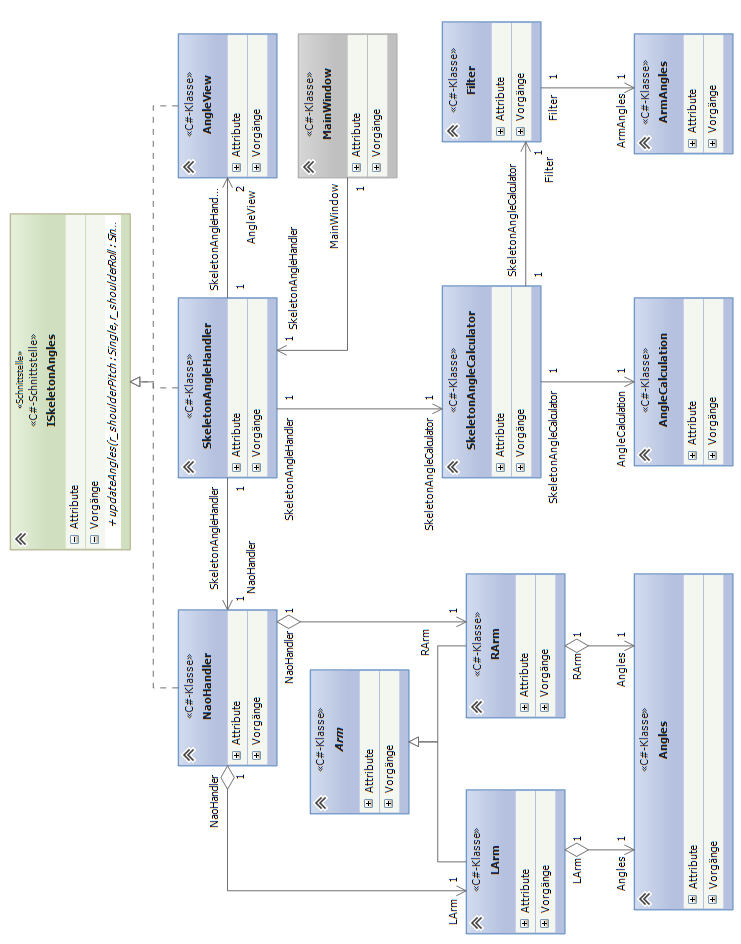
\includegraphics[scale=0.8]{Bilder/classdiagramm.png}
	\caption{UML - Klassendiagramm}						
	\label{f:classdiagramm}						
\end{figure}

\subsection{MainWindow}
Die C\# Applikation wird als WPF-Anwendung gestartet. Dies geschieht in der Klasse \textbf{MainWindow}. Hierbei werden alle Parameter initialisiert und alle nötigen Objekte erzeugt, wie der KinectSensor und der KinectHandler. Es wird wie in Kapitel ...SDK... beschrieben, der Tiefenstream und der Skeletonstream der Kinect aktiviert und anschließend ein "AllFramesReady"-Event registriert, das benutzt wird, sobald ein Skelett vor der Kamera vollständig erkannt wurde. Im Eventhandler wird der Berechnungs-Handler mit der aktuellen Position des gefilterten Skelettes versorgt. Zudem wird die GUI mit dem aktuellen RGB-Bild aktualisiert und erhält noch ein Skelett-Overlay, sodass man auch im Fenster sehen kann, dass ein Skelett erkannt wurde und kann dieses betrachten. Eine weitere Funktion dieser Klasse ist, das kontrollierte Beenden der Applikation. Nach schließen des Programmes, werden alle Berechnungen gestoppt, die Handler heruntergefahren und Kinect ausgeschaltet.



\subsection{SkeletonAngleHandler}
Der \textbf{AngleHandler} löst verschiedene Aufgaben. Zunächst erzeugt er in der Initialisierungsphase zwei Fenster, die in den späteren Phasen die errechneten Winkel ausgeben. Für jede Seite (rechts, links) wird ein Fenster erzeugt, das alle 4 relevanten Winkel enthält. Des Weiteren wird ein Thread erzeugt, der für die Errechnung der Winkelwerte aus dem ausgelesenen Skelett zuständig ist. Da diese Aktion relativ rechenintensiv ist, wurde sie in einen eigenen Thread ausgelagert. Zudem wird während der Initialisierungsphase der NaoHandler erzeugt, der für die spätere Übertragung und Transformation der errechneten Werte an den Roboter zuständig ist.
Der Handler selbst verfügt über eine Liste mit Beobachtern, die informiert werden, falls eine neue Berechnung erfolgt ist. Beobachter sind konkret die beiden Fenster für die Debugging-Ausgabe und der Nao-Handler. Hierbei könnte somit dynamisch nach Bedarf noch ein neuer Beobachter hinzugefügt werden, der die Winkelwerte der menschlichen Pose verwenden könnte.
Der Handler selbst wird durch das Event \textbf{AllFramesReady} in der Klasse MainWindow über seine Methode \textbf{updateSkeleton} benachrichtigt und erhält ein neu erkanntes Skelett. Dieses gibt er an den Berechnungsthread weiter, der eine neue Berechnung startet. Nach erfolgreicher Berechnung werden alle Beobachter über die neuen Werte informiert. 

%
%	Problem/Besonderheit
%		Es musste eine eigene Klasse zur Beendigung implementiert werden, da sonst 
%		Speicherverletzungen
%		beim Beenden entstehen -> Known Issue bei Microsoft
%

\subsection{SkeletonAngleCalculator}
Diese Klasse erhält als Input ein Skelett, lässt die vier benötigten Armwinkel berechnen und gibt diese zurück an den Handler. Die Berechnung erfolgt durch den statischen Aufruf der Factory-Klasse \textbf{AngleCalculation}. Diese enthält den Algorithmus, der mittels Skalarprodukt die Armstellungen errechnet. (Siehe Kapitel XYZ). Nach der Errechnung werden die Gelenkstellungen noch durch einen Medianfilter geschickt. Dieser soll extreme Schwankungen der Kinect-Erkennung ausschließen.

\subsection{NaoHandler}
Die Klasse \textbf{NaoHandler} ist sozusagen der Output der Anwendung. In dieser Klasse wird die Kommunikation zu Nao erzeugt und aufrecht erhalten. Ferner wird das Interface \textbf{ISkeletonAngles} implementiert und somit die Aktualisierung der Armwinkel durchgeführt. Es wird jeweils ein Arm für Rechts und Links erzeugt. Die Winkel nimmt sie entgegen und delegiert die Umrechnung an den jeweiligen Arm. Die tatsächliche Umwandlung der Winkel in den Nao - Gelenkraum und die Überprüfungen werden im jeweiligen Arm spezifiziert (siehe \myref{s:naoAlgo}). Zusätzlich sorgt sie dafür, dass sich der Roboter bei Beendigung der Anwendung in die sichere Pose \textit{Sitzen} begibt.



\subsection{Interfaces}
Als Schnittstelle zwischen der Erkennung und der Ausführung der Armpositionen wird essenziell die Methode \textit{updateAngles} vom Interface \textit{ISkeletonAngles} verwendet. Diese stellt alle benötigten Winkel wie Shoulder Pitch, Shoulder Roll, Ellbow Roll, Elbow Yaw bereit. Somit kann dieses Interface von allen Klassen implementiert werden, die immer die aktuellen Werte benötigen, wie der NaoHandler und die GUI.


\subsection{Flussdiagramm: Winkelerkennung}
	\begin{figure}[H]						
		\centering							
		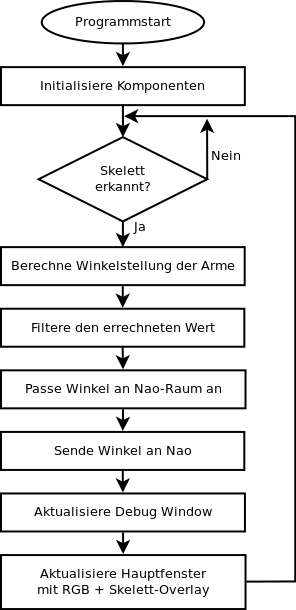
\includegraphics[scale=0.8]{Bilder/Flussdiagramm.png}			
		\caption{Programmablauf: Winkelerkennung}						
		\label{f:pap}						
	\end{figure}
